\chapter{From Static Reasoning to Embodied Action}
\label{sec:embodied}

\section{Why Embodied Evaluation Matters}

The two papers established that (a) spatial intelligence is a major weakness of current models and (b) data scaling can substantially improve it on static benchmarks. But a deeper question remained, namely \textit{do these improvements matter for agents that must act in the world?}

Static benchmarks test spatial reasoning in isolation, where the model simply sees images, reads a question, and produces text. An embodied agent, by contrast, must close the loop by perceiving the environment, reasoning about its spatial structure, deciding on an action, executing it, observing the consequences, and planning the next step. This loop introduces entirely new failure modes. An agent might have perfect spatial perception but poor planning, or excellent reasoning but no ability to recover when an action fails.

A preliminary result from the SenseNova-SI paper~\cite{cai2025scalingspatialintelligencemultimodal} hinted at the connection. Applying SenseNova-SI to EmbodiedBench manipulation tasks \textit{without any fine-tuning} produced measurable performance improvements, suggesting that spatial data scaling benefits extend beyond static Q\&A. But this was tested on only one domain with one benchmark. A systematic investigation would require running diverse embodied benchmarks under controlled conditions, and no unified framework for doing so existed.

\section{Designing the EASI Embodied Evaluation Library}

To enable this investigation, I independently designed and built the EASI embodied evaluation library, extending the EASI evaluation philosophy from static benchmarks to interactive simulator-based evaluation. The library addresses a practical challenge that had long fragmented the embodied AI community. Each simulator (AI2-THOR, Habitat-Sim, CoppeliaSim, ThreeDWorld) has its own Python version requirements, GPU dependencies, API conventions, and episode formats. Running even a single benchmark often required days of environment debugging; running multiple benchmarks for comparative evaluation was a research project in itself.

Figure~\ref{fig:architecture} shows the high-level architecture. The library is organized around four key capabilities, each addressing a concrete barrier to systematic embodied evaluation.

\begin{figure}[htbp]
\centering
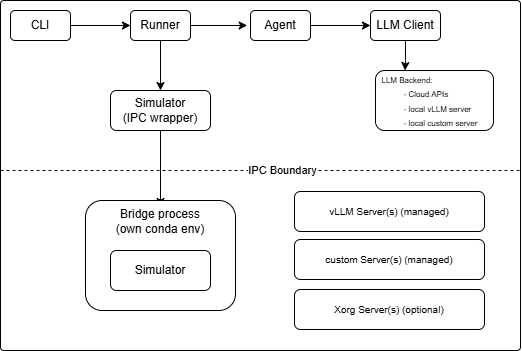
\includegraphics[width=0.7\textwidth]{fig/easi_arch.png}
\caption{High-level architecture of the EASI embodied evaluation library. The subprocess boundary separates the host process (Python 3.10+) from simulator bridge processes that may run different Python versions. Communication uses atomic JSON file I/O. See Appendix~\ref{sec:appendix_architecture} for detailed process flow.}
\label{fig:architecture}
\end{figure}

\subsection{Unified Multi-Simulator Evaluation}

The core architectural insight is \textbf{subprocess isolation}. Each simulator runs in its own conda environment, potentially with a different Python version. AI2-THOR v2.1 requires Python 3.8, Habitat-Sim requires Python 3.9, while the host runs Python 3.10+. A bridge script inside each simulator's environment communicates with the parent process through filesystem-based IPC, using atomic JSON file reads and writes in a temporary directory. This avoids the complexity of socket-based communication while maintaining reliability across Python version boundaries. The IPC protocol uses three files (\texttt{status.json}, \texttt{command.json}, and \texttt{response.json}) with atomic writes via rename to prevent partial reads (see Appendix~\ref{sec:appendix_ipc}).

On top of this isolation layer, the library provides a unified interface. A single CLI command (\texttt{easi start}) with a task name, agent type, backend, and model works identically across all benchmarks. Tasks are auto-discovered via YAML configuration files; simulators are registered through manifest files. Adding a new benchmark requires only a task directory with a YAML config and a Python class, with no modification to any central registry. For benchmarks with multiple evaluation splits (EmbodiedBench has 19 splits across four domains), YAML template inheritance keeps configuration DRY, where split-specific configs extend a shared base via \texttt{extends:~\_base.yaml}, varying only the dataset subset, episode filter, or action space.

\subsection{Standardised Agent-Environment Interface}

A key challenge in embodied evaluation is that different benchmarks require different prompt formats, action spaces, and feedback mechanisms. The library addresses this through a \textbf{PromptBuilder} protocol that standardises the agent-environment interface while remaining customisable per benchmark.

The standard prompt format uses a two-message structure as shown in Figure~\ref{fig:prompt_structure}. The system prompt follows a fixed section order (Role and Environment, Available Actions, Strategy, Guidelines, and Response Format), providing the LLM with a consistent frame of reference regardless of which benchmark is running. The user message assembles per-step dynamic content, including the current camera image, task instruction, environment feedback (e.g., geodesic distance to goal), and a truncated action history showing previous actions and their outcomes. A complete prompt example for a navigation episode is provided in Appendix~\ref{sec:appendix_prompt}.

\begin{figure}[htbp]
\centering
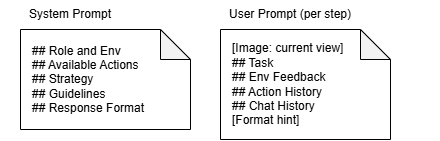
\includegraphics[width=0.7\textwidth]{fig/prompt.png}
\caption{Standardised prompt structure. The system prompt is static per benchmark; the user message is assembled fresh each step with current observations and history.}
\label{fig:prompt_structure}
\end{figure}

The LLM responds in a standardised 4-field JSON format: a visual state description, reasoning and reflection, a language plan, and an executable plan containing a list of actions. This structured format enables \textit{multi-action buffering}. When the LLM generates a plan with multiple actions, the agent executes them one at a time without re-prompting the LLM until an action fails or the buffer is exhausted, substantially reducing API calls.

\subsection{Scalable Parallel Evaluation}

Embodied evaluation is time-intensive. A single EB-Alfred episode may involve 50+ LLM calls with image inputs, and a full benchmark can take hours to complete sequentially. To make large-scale evaluation practical, the library supports \textit{thread-pool parallelism} where each worker gets its own simulator process, agent instance, and LLM client. Workers pull episodes from a shared thread-safe queue, enabling automatic load balancing.

For local inference using vLLM, the library manages the full server lifecycle. A \texttt{MultiServerManager} spawns multiple vLLM instances across designated GPUs using a two-phase startup (spawn all processes, then concurrent health checks), distributes workers across instances via round-robin URL assignment, and tears down servers on completion. GPU allocation is explicitly partitioned into separate pools for LLM inference and simulator rendering, preventing resource contention. A render platform abstraction handles the diverse display requirements of different simulators, supporting six backends (native X11, virtual framebuffer, EGL headless, managed Xorg, and others) with per-worker GPU binding. See Appendix~\ref{sec:appendix_parallel} for detailed worker lifecycle and resource management.

\subsection{Reproducibility and Analysis}

Long-running evaluations need robust support for interruption and resumption. The library saves a configuration file with all CLI options at run start, and each completed episode writes its metrics and step-by-step trajectory (including observation images) to a structured output directory. A resume flag restarts from the last completed episode, re-aggregating results across both completed and new episodes.

An episode filtering syntax supports index ranges, specific episode IDs, and mixed specifications, enabling targeted re-evaluation of particular episodes without rerunning the full benchmark.

\section{The Breadth of Embodied Evaluation}

Before implementing the library's architecture, I had spent several weeks verifying each of the EmbodiedBench~\cite{yang2025embodiedbenchcomprehensivebenchmarkingmultimodal} environments (Alfred, Navigation, Habitat, and Manipulation), setting up their respective simulators on the server and confirming that episodes could be loaded, reset, and stepped through correctly. This groundwork informed the library's design and ensured that the abstractions I chose would accommodate the real diversity of simulator interfaces.

The library now integrates ten embodied benchmarks spanning five simulators and a wide range of capabilities.

EmbodiedBench's four domains alone cover 19 evaluation splits. \textbf{EB-Alfred} (AI2-THOR v2.1) tests household task completion across six capability dimensions, namely base, spatial, visual, commonsense, complex instruction following, and long-horizon planning. A ``complex'' episode might require the agent to execute 20+ sequential actions (``heat the potato, then put it on the counter, then pick up the knife\ldots''), while a ``spatial'' episode tests whether the agent can locate objects based on spatial descriptions. \textbf{EB-Navigation} (AI2-THOR v5.0) evaluates indoor point-goal navigation with five splits. \textbf{EB-Habitat} (Habitat-Sim) tests scene understanding combined with navigation across four splits. \textbf{EB-Manipulation} (CoppeliaSim) evaluates robotic manipulation, specifically precise 3D gripper positioning using discrete action coordinates.

Beyond EmbodiedBench, the library integrates \textbf{HAZARD}~\cite{zhou2024hazardchallengeembodieddecision} (ThreeDWorld), which presents a qualitatively different challenge. The agent must infer \textit{implicit} goals under emergency conditions. During a fire scenario, the agent is not told ``evacuate the laptop'' but instead must reason that valuable objects should be rescued and identify which objects are valuable, all while navigating a dynamically changing environment. This tests what I term \textit{situational goal reasoning}, a capability not captured by any static benchmark.

\textbf{ManipulaTHOR}~\cite{ehsani2021manipulathorframeworkvisualobject} tests arm-based point navigation in AI2-THOR, and \textbf{AI2-THOR Rearrangement 2023}~\cite{RoomR} evaluates an agent's ability to restore objects to their original positions across five evaluation splits. The \textbf{VLN-CE}~\cite{krantz2020navgraphvisionandlanguagenavigationcontinuous} benchmarks (R2R and RxR) bring vision-and-language navigation into continuous environments using Habitat-Sim, requiring agents to translate free-form natural language instructions (``Walk past the dining table, turn left at the hallway, stop at the second door on your right'') into continuous movement. The RxR variant includes Hindi and Telugu instructions, enabling multilingual embodied evaluation. \textbf{LHPR-VLN}~\cite{song2025longhorizonvisionlanguagenavigationplatform} extends this with multi-subtask navigation requiring hierarchical planning.

\section{The LLM-Driven Agent}

To drive evaluation across these diverse benchmarks, the library implements an LLM-driven agent that follows a perceive-reason-act loop. At each step, the agent receives an egocentric camera image and environment feedback from the simulator. It maintains an \textbf{agent memory} that tracks the full interaction history, including previous observations, actions taken, environment feedback received, and the LLM's own prior responses, providing the context needed for coherent multi-step behaviour. The PromptBuilder (Section~\ref{sec:embodied}) assembles this memory into a structured prompt, which is sent to the LLM for reasoning. The LLM returns a structured response containing its visual description of the scene, reasoning about the current situation, a natural language plan, and one or more proposed actions. The agent validates each action against the task's action space and executes them sequentially.

Two mechanisms make this loop practical at scale. First, \textbf{multi-action buffering}. When the LLM generates a plan with multiple actions, the agent executes them one at a time without re-prompting the LLM until an action fails or the buffer is exhausted, substantially reducing API calls. Second, \textbf{feedback-driven replanning}. When an action fails, the failure is recorded in the action history, the action buffer is cleared, and the agent re-prompts the LLM with the updated context on the next step. This enables error recovery without explicit failure-handling logic. The LLM reasons about what went wrong based on the feedback history and adjusts its plan accordingly.

The agent interface is pluggable as the current implementation uses an LLM for reasoning, but the library also includes a dummy agent (random action selection) for testing, and the protocol is designed so that alternative agent architectures, such as those incorporating explicit spatial maps or hierarchical planners, can be substituted without modifying the evaluation pipeline.

\section{What Embodied Evaluation Adds to the Picture}

The capability dimensions tested by embodied benchmarks partially overlap with the EASI static taxonomy but extend it in important ways. Static benchmarks test whether a model can answer \textit{``which object is to the left of the chair?''}, while embodied benchmarks test whether an agent can \textit{navigate to} the left of the chair, pick up the object there, and carry it to another room. This requires not just spatial perception (SR) and perspective-taking (PT), but also the following.

\begin{itemize}
    \item \textbf{Long-horizon planning}: Decomposing complex goals into executable action sequences, maintaining a mental model of progress, and deciding when to replan.
    \item \textbf{Situational goal reasoning}: Inferring what to do when the goal is not explicitly stated (HAZARD scenarios).
    \item \textbf{Grounded language understanding}: Translating natural language navigation instructions into continuous movement through 3D space (VLN-CE).
    \item \textbf{Error recovery}: Detecting when an action has failed (a gripper didn't close, a navigation step was blocked) and adapting the plan accordingly.
\end{itemize}

The preliminary finding from~\cite{cai2025scalingspatialintelligencemultimodal}, that SenseNova-SI improved EmbodiedBench manipulation performance without fine-tuning, is encouraging. The EASI embodied library now makes it possible to test this transfer systematically across all ten benchmarks and multiple model families, providing a much richer picture of whether and how static spatial intelligence translates to embodied competence.

\section{Preliminary Experiment: EASI-Mini}

To provide an initial data point on whether static spatial intelligence gains transfer to embodied settings, I designed and ran a compact cross-benchmark evaluation called EASI-Mini. The benchmark samples 74 episodes across six capability dimensions from the library's integrated benchmarks, enabling a structured comparison without the cost of running all ten benchmarks at full scale.

The benchmark is designed such that each capability dimension draws episodes from one or more source benchmarks, as summarised in Table~\ref{tab:easimini_design}. Episodes are sampled deterministically (seed 42) for reproducibility. Success is normalized across benchmarks, using \texttt{task\_success} for EmbodiedBench and \texttt{success} (within 3m of goal) for VLN-CE.

\begin{table}[htbp]
\centering
\caption{EASI-Mini benchmark design: capability dimensions and episode sources.}
\label{tab:easimini_design}
\renewcommand{\arraystretch}{1.1}
\small
\begin{tabular}{lp{4.5cm}r}
\toprule
\textbf{Capability} & \textbf{Sources} & \textbf{Eps} \\
\midrule
Spatial Reasoning & EB-Alfred, EB-Habitat, EB-Manipulation & 9 \\
Common Sense & EB-Alfred, EB-Navigation, EB-Habitat, EB-Manipulation & 12 \\
Complex Instruction & EB-Alfred, EB-Navigation, EB-Habitat, EB-Manipulation & 12 \\
Long-Horizon Planning & EB-Alfred, EB-Habitat, LHPR-VLN & 14 \\
Visual Grounding & EB-Alfred, EB-Navigation, EB-Habitat, EB-Manipulation & 12 \\
Continuous Navigation & VLN-CE R2R (val unseen) & 15 \\
\midrule
\textbf{Total} & & \textbf{74} \\
\bottomrule
\end{tabular}
\end{table}

For model evaluation, four models were selected to span the proprietary--open-source axis and to test the effect of spatial data scaling. \textbf{GPT-5.2} serves as a proprietary baseline with strong general vision capabilities. \textbf{Qwen3-8B-Instruct} is a competitive open-source model from the static evaluation (Chapter~\ref{sec:diagnosis}). \textbf{InternVL3-8B} provides the base model before spatial data scaling, while \textbf{SenseNova-SI InternVL3-8B} is the same model after SFT on SenseNova-SI-8M spatial data as described in Chapter~\ref{sec:treatment}.

The InternVL3-8B vs.\ SenseNova-SI InternVL3-8B comparison directly tests the central question of whether the dramatic improvement on static spatial benchmarks (e.g., 41.5\% $\to$ 85.6\% on MindCube) translates into better embodied performance.

\begin{table}[htbp]
\centering
\caption{EASI-Mini results: success rate (\%) by capability dimension.}
\label{tab:easimini_capability}
\renewcommand{\arraystretch}{1.1}
\begin{tabular}{lcccc}
\toprule
\textbf{Capability} & \textbf{GPT-5.2} & \textbf{Qwen3-8B} & \textbf{InternVL3-8B} & \textbf{SN-SI InternVL3-8B} \\
\midrule
Spatial Reasoning & 33.3 & 11.1 & 11.1 & 0.0 \\
Common Sense & 41.7 & 16.7 & 8.3 & 0.0 \\
Complex Instruction & 33.3 & 16.7 & 16.7 & 8.3 \\
Long-Horizon Planning & 28.6 & 0.0 & 0.0 & 0.0 \\
Visual Grounding & 58.3 & 25.0 & 16.7 & 0.0 \\
Continuous Navigation & 33.3 & 0.0 & 6.7 & 0.0 \\
\midrule
\textbf{Overall} & \textbf{37.8} & \textbf{10.8} & \textbf{9.5} & \textbf{1.4} \\
\bottomrule
\end{tabular}
\end{table}

\begin{table}[htbp]
\centering
\caption{EASI-Mini results: success rate (\%) by source benchmark.}
\label{tab:easimini_benchmark}
\renewcommand{\arraystretch}{1.1}
\begin{tabular}{lcccc}
\toprule
\textbf{Benchmark} & \textbf{GPT-5.2} & \textbf{Qwen3-8B} & \textbf{InternVL3-8B} & \textbf{SN-SI InternVL3-8B} \\
\midrule
EB-Alfred & 66.7 & 13.3 & 0.0 & 0.0 \\
EB-Navigation & 66.7 & 22.2 & 22.2 & 11.1 \\
EB-Habitat & 6.7 & 0.0 & 0.0 & 0.0 \\
EB-Manipulation & 41.7 & 33.3 & 33.3 & 0.0 \\
VLN-CE R2R & 33.3 & 0.0 & 6.7 & 0.0 \\
LHPR-VLN & 12.5 & 0.0 & 0.0 & 0.0 \\
\bottomrule
\end{tabular}
\end{table}


\textbf{Analysis.} The results reveal a clear model capability hierarchy. GPT-5.2 (37.8\% overall SR) substantially outperforms all open-source models, followed by Qwen3-8B (10.8\%), InternVL3-8B (9.5\%), and SenseNova-SI InternVL3-8B (1.4\%). Several patterns stand out.

\textbf{Spatial SFT degrades instruction following.} The central question of this experiment was whether SenseNova-SI's dramatic gains on static spatial benchmarks (e.g., 41.5\% $\to$ 85.6\% on MindCube) would translate into better embodied performance. SenseNova-SI InternVL3-8B (1.4\% SR) actually underperforms the base InternVL3-8B (9.5\% SR) across nearly all capability dimensions and benchmarks. However, this does not necessarily mean spatial data scaling is ineffective for embodied tasks. Analysis of the failure modes reveals that the dominant cause of failure is the model's inability to generate well-formed JSON action outputs, leading to parse errors and zero-step episodes. The spatial SFT appears to have degraded the model's instruction-following and structured output capabilities rather than its spatial reasoning per se. Several open-source models, particularly on EB-Manipulation and EB-Habitat, completed episodes with zero steps taken for this reason. Future work on spatial data curation should consider preserving instruction-following ability during SFT, perhaps through mixed training with general-purpose data.

\textbf{Proprietary models hold a decisive advantage.} GPT-5.2 leads across every capability dimension and every benchmark. The gap is particularly large on EB-Alfred (66.7\% vs 13.3\% for the next best) and EB-Navigation (66.7\% vs 22.2\%), both of which require multi-step planning and structured action output. This suggests that embodied tasks benefit from capabilities beyond spatial perception, including instruction following, action grounding, and error recovery, where larger proprietary models excel.

\textbf{Long-horizon planning is the weakest capability.} Across all models, long-horizon planning and continuous navigation yield the lowest success rates, while visual grounding is consistently the strongest (58.3\% for GPT-5.2, 25.0\% for Qwen3-8B). One contributing factor may be the evaluation setup. The current agent uses only action history (previous actions and their outcomes) but not full chat history (the model's own prior reasoning). Without access to its earlier reasoning traces, the model cannot build on previous plans or maintain coherent long-term strategies, which disproportionately affects tasks requiring many sequential steps.

This experiment is preliminary. Each capability dimension samples only 3 to 5 episodes per benchmark. The small sample sizes limit statistical robustness, and the results should not be treated as definitive assessments of model capability. Nevertheless, EASI-Mini demonstrates the library's ability to produce structured, cross-benchmark comparisons with a single evaluation script, and provides an initial signal on the static-to-embodied transfer question.
